%% img/NPClass/CLIHCLI1.tex
%% Copyright 2019 Andrea Berlingieri
%
% This work may be distributed and/or modified under the
% conditions of the LaTeX Project Public License, either version 1.3
% of this license or (at your option) any later version.
% The latest version of this license is in
%   http://www.latex-project.org/lppl.txt
% and version 1.3 or later is part of all distributions of LaTeX
% version 2005/12/01 or later.
%
% This work has the LPPL maintenance status `maintained'.
%
% The Current Maintainer of this work is Andrea Berlingieri.
%
% This work consists of all files listed in manifest.txt
\documentclass{standalone}

\usepackage{../TikzStyle}
\usepackage{../mystyle}
%\usetikzlibrary{decorating}
\usetikzlibrary{positioning}

\newcommand{\GraphG}[3]{% x,y,name
    \node[point] (#3_m1) at ([shift={(#1 cm,#2 cm)}]0,0) {};
    \node[point] (#3_m2) at ([shift={(#1 cm,#2 cm)}]0.69,-1.2) {};
    \node[point] (#3_m3) at ([shift={(#1 cm,#2 cm)}]-0.69,-1.2) {};
    \node[point] (#3_m4) [above=0.75cm of #3_m1] {};
    \draw (#3_m1) -- (#3_m2) -- (#3_m3) -- (#3_m1) -- (#3_m4);
}

\begin{document}
    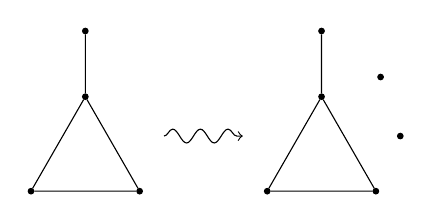
\begin{tikzpicture}[point/.style={draw,circle,inner sep=0cm,fill=black,minimum size=2pt}]
        \GraphG{0}{0}{G}
        \draw[decorate,decoration=snake,->] (1,-0.5) -- (2,-0.5);
        \GraphG{3}{0}{G2}
        \node[point] () at (3.75,0.25) {};
        \node[point] () at (4,-0.5) {};
    \end{tikzpicture}
\end{document}
